\subsection{Normalizing}
In addition to comparing all motif importance values within the same cluster, the goal is also to compare individual motifs importance values across clusters. As such it is necessary to normalize $x_{C_\kappa,m}$ in order to elucidate subtle differences across all relevant cluster criteria. One simple and effective option is to use the standard score $z_{C_\kappa,m}$.

In a realistic analysis, the number of clusters is generally very small. For example, if $\kappa \in \left\{patient\ is\ taking\ an\ SSRI,patient\ is\ not\ taking\ an\ SSRI\right\}$, then the mean $\mu_{.,m}$ and standard deviation $\sigma_{.,m}$ of importance values for motif $m$ across all clusters in the analysis only take into account two values for $x_{C_\kappa,m}$, hardly enough to calculate a useful standard score. Therefore, instead of normalizing values of $x_{.,m}$ directly against each other, values of $x_{C_\kappa,m}$ were normalized against the random distribution $x_{C_\kappa,m}^*$, bootstrapped by taking a sufficiently large number of random samples of relative importance values. For any given cluster $C_\kappa$ and motif $m$,

\begin{enumerate}
  \item Let $|C_\kappa|$ be the number of patients in $C_\kappa$.
  \item Take some arbitrarily large number $n$ (say, 1000) of random samples $\left(C_{r_1},...,C_{r_n}\right)$ so that each sample represents a cluster of $|C_\kappa|$ patients independently chosen from $\left\{all\ patients\right\}$ with replacement and uniform probability of being chosen.
  \item For each sample $C_r$, calculate the relative motif importance $x_{C_r,m}$. Refer to this new set, $\left\{x_{C_{r_1},m}, x_{C_{r_2},m}, ..., x_{C_{r_n},m}\right\}$, as $x_{C_\kappa,m}^*$. Ideally $x_{C_\kappa,m}^*$ will resemble a normal distribution. As figure \ref{fig:5x5_hist} shows, this appears to be the case from the data set for example values of $n_r=1000$, $|C_\kappa|=100$, and $\beta=5$. Although, this is not necessarily the case for every $x_{C_\kappa,m}^*$ when $\beta$ is sufficiently large or $|C_\kappa|$ is sufficiently small. Figure \ref{fig:10x10_hist_ck100} shows $x_{C_\kappa,m}^*$ histograms when $n_r=1000$, $|C_\kappa|=100$, and $\beta=10$. Near two of the corners $x_{C_\kappa,m}^*$ values hover around 0. The reason is that instances of such drastic jumps in pain scores (\emph{j} to \emph{a} or \emph{a} to \emph{j}) are relatively rare. For practical purposes, the visual effect on the final icons as well as the effect on sorting the icons is negligible, so this small source of normalization error is acceptable. However, figure \ref{fig:10x10_hist_ck2} shows $x_{C_\kappa,m}^*$ histograms when $n_r=1000$, $|C_\kappa|=2$, and $\beta=10$. Data calculated for these parameters are clearly not normal, which is unsurprising given that the numerator in $x_{C_\kappa,m}$ expresses additive behavior over potentially rare events; that is, the sum of the number of times patients in a given cluster went from one normalized pain level to another. Therefore, in this analysis, which limited $\beta$ to a maximum value of 10, only clusters which contained at least 100 patients ($|C_\kappa|\geq100$) were considered. As it turns out, most interesting clusters have several hundred patients, so this limit is rarely an issue. In the future, however, other probability distributions may prove useful in analyzing these smaller clusters.
\begin{figure}
  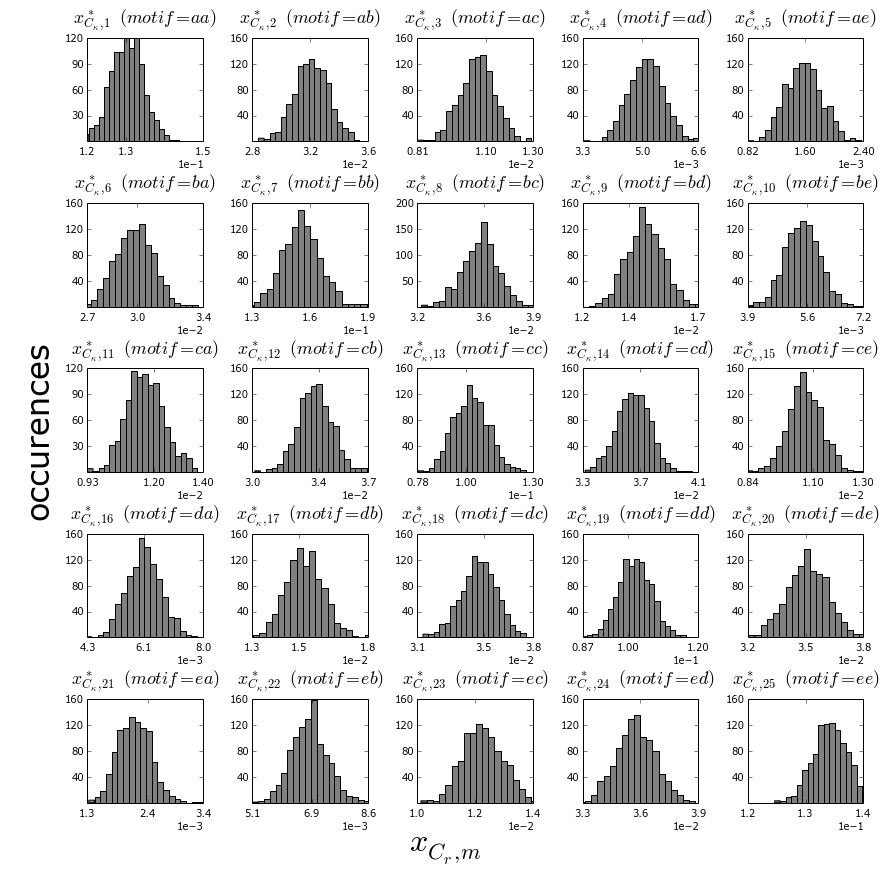
\includegraphics[scale=0.35]{./Figures/5x5hist.png}\\
  \caption{Histograms of resampled importance values for each motif, with parameters $n_r=1000$, $|C_\kappa|=100$, and $\beta=5$. Demonstrates ideal normal behavior of the simulated importance value distributions.}\label{fig:5x5_hist}
\end{figure}
\begin{figure}
  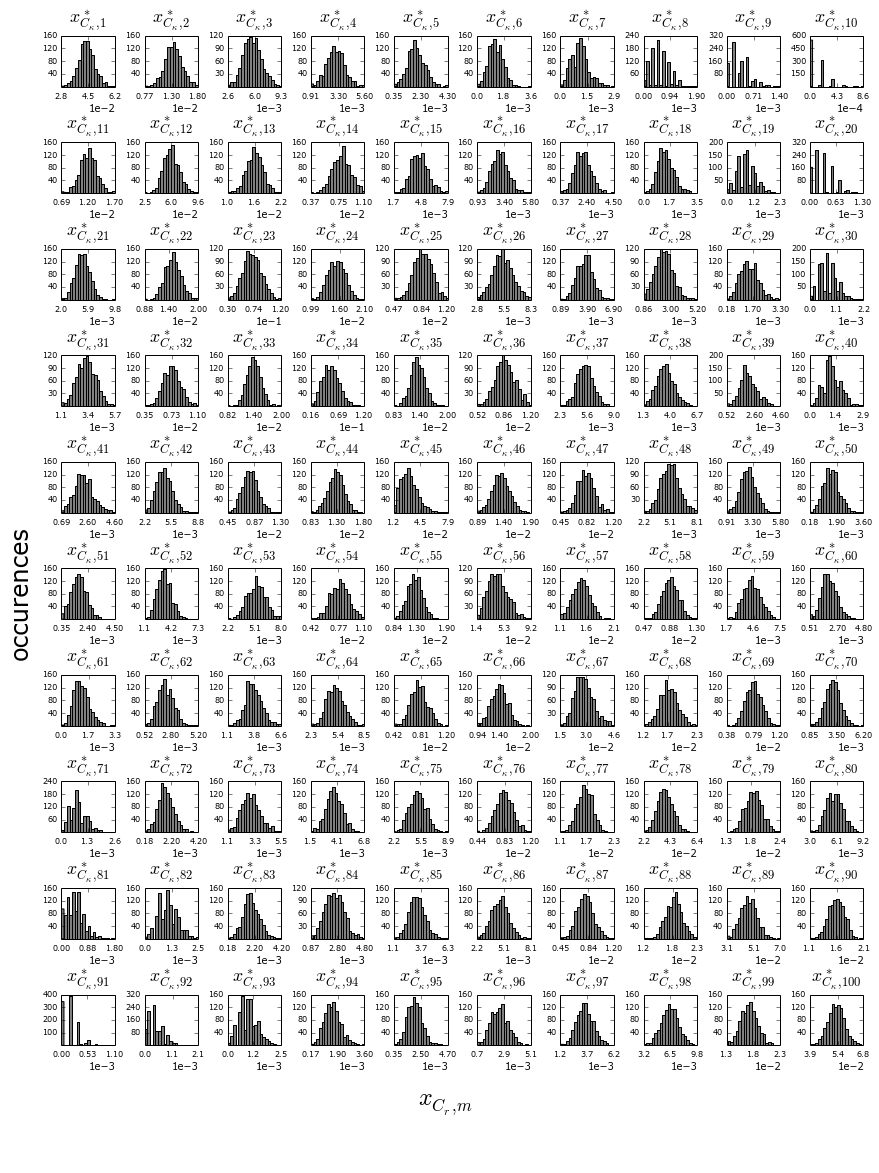
\includegraphics[scale=0.35]{./Figures/10x10hist_ck100.png}\\
  \caption{Histograms of resampled importance values for each motif, with parameters $n_r=1000$, $|C_\kappa|=100$, and $\beta=10$. Demonstrates slight deviation from normal behavior around the upper-right and lower-left corners.}\label{fig:10x10_hist_ck100}
\end{figure}
\begin{figure}
  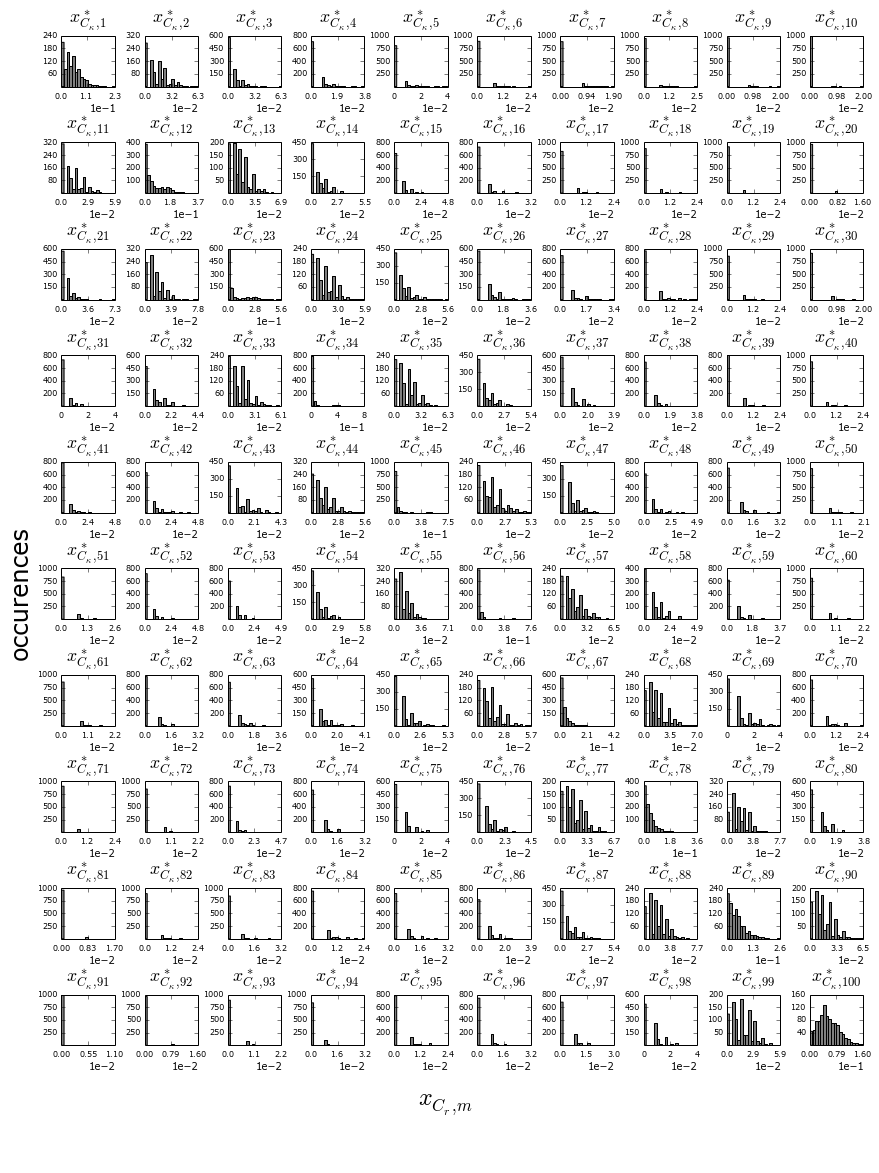
\includegraphics[scale=0.35]{./Figures/10x10hist_ck2.png}\\
  \caption{Histograms of resampled importance values for each motif, with parameters $n_r=1000$, $|C_\kappa|=2$, and $\beta=10$. Demonstrates collapse of normality expectation and necessitates the restriction on cluster sizes of less than 100 patients.}\label{fig:10x10_hist_ck2}
\end{figure}
  \item From $x_{C_\kappa,m}^*$, calculate the mean $\mu_{C_\kappa,m}$ and standard deviation $\sigma_{C_\kappa,m}$. The normalized value of $x_{C_\kappa,m}$ is therefore the standard score

\begin{equation}\label{eqn:normalize_motif_importance}
    z_{C_\kappa,m}=\frac{x_{C_\kappa,m}-\mu_{C_\kappa,m}}{\sigma_{C_\kappa,m}}
\end{equation}

      The vertical lines in figure \ref{fig:5x5hist_standardscore} represent values for $z_{C_\kappa,m}$ plotted against histograms for standard scores of all values in $x_{C_\kappa,m}^*$; that is, equation \eqref{eqn:normalize_motif_importance} applied to all sampled points in $x_{C_\kappa,m}^*$ (creating a derived distribution, $z_{C_\kappa,m}^*$). Specifically, these data represent parameter values $\beta=5$, $n_r=1000$, and $\kappa=$``\emph{patient underwent cardiovascular surgery}'' (PrimaryCPTCodeCategory2 = \emph{Cardiovascular}), a cluster which contains 582 patients ($|C_\kappa|=582$).

\begin{figure}
  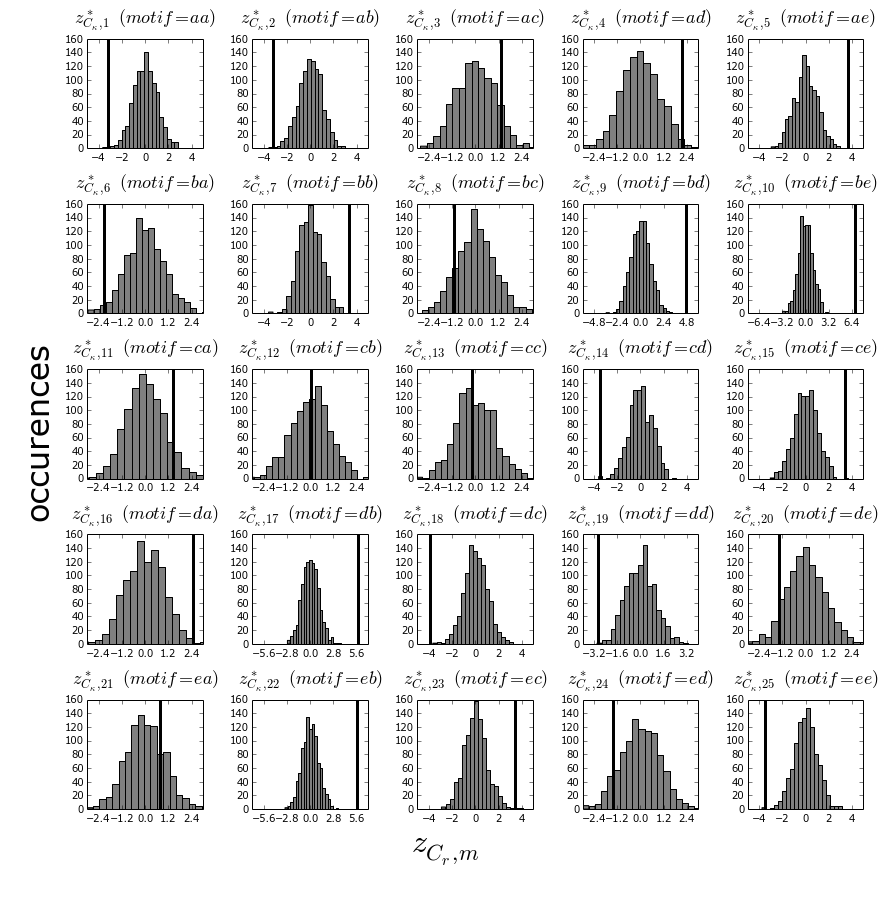
\includegraphics[scale=0.35]{./Figures/5x5hist_standardscore.png}\\
  \caption{Histograms of resampled importance values for each motif, converted to their standard score, with parameters $n_r=1000$, $|C_\kappa|=100$, and $\beta=5$. Vertical lines correspond to normalized importance values for the cluster of patients that underwent cardiovascular surgery.}\label{fig:5x5hist_standardscore}
\end{figure}

\end{enumerate} 